\documentclass[11pt]{jsk-thesis}

%レイアウト補正
%\usepackage{layout}
%\setlength \voffset {-1.0cm}
%\setlength \hoffset {-1.2cm}
%\setlength \textwidth {17cm}
%\setlength \textheight {24cm}

%パッケージ読み込み
\usepackage[dvipdfmx]{graphicx}
\usepackage[dvipdfmx]{color}
\usepackage{booktabs}
\usepackage{amsmath}
\usepackage{amssymb}
\usepackage{bm}
\usepackage{url}

%コマンド定義
%表の日付のフォントサイズ変更
\newcommand{\tdate}[1]{\scriptsize{#1}}
%単位"°"
%%\newcommand{\degree}[1]{#1^{\circ}}
%微分演算子関係
\newcommand{\dd}{\mathrm{d}}
\newcommand{\diff}[2]{\frac{\mathrm{d}#1}{\mathrm{d}#2}} %常微分
\newcommand{\diffline}[2]{\mathrm{d}#1/\mathrm{d}#2} %文章中での常微分
\newcommand{\ddiff}[3]{\frac{\mathrm{d}^#1 #2}{\mathrm{d} #3^#1}} %高階常微分
\newcommand{\ddiffline}[3]{\mathrm{d}^#1 #2/\mathrm{d} #2^#1} %文章中での高階常微分
\newcommand{\pdiff}[2]{\frac{\partial #1}{\partial #2}} %偏微分
\newcommand{\pddiff}[3]{\frac{\partial^#1 #2}{\partial #3^#1}} %高階偏微分
\newcommand{\non}[1]{#1^{*}} %無次元化変数

%関数
\newcommand{\erf}{\mathrm{erf}}

%その他
\newcommand{\myfig}[5]{
  \begin{figure}[#1]%
    \begin{center}%
      \includegraphics[width=#2]{#3}%
      \caption{#4}%
      \label{fig:#5}%
    \end{center}%
  \end{figure}%
}
%% \newcommand{\figref}[1]{Fig.\ref{fig:#1}}
%% \newcommand{\seclabel}[1]{\label{sec:#1}}
%% \newcommand{\secref}[1]{第{\bf\ref{sec:#1}}節}

\newcommand{\unit}[1]{\,[\mathrm{#1}]}

%見出し変更
\renewcommand{\figurename}{Fig.}
\renewcommand{\tablename}{Table}



\usepackage{ikuo}%%便利コマンド集.



\usepackage[dvipdfmx]{hyperref}  % 目次や参考文献をリンクにする。
\usepackage{pxjahyper} %% これを入れるとしおりが文字化けしない。out2uniが不要になる。
%% \hypersetup{bookmarksnumbered=true}
\hypersetup{colorlinks=true}
\hypersetup{linkcolor=black}
%% \hypersetup{linkbordercolor=black}
\hypersetup{urlcolor=black}
%% \hypersetup{urlbordercolor=black}
\hypersetup{citecolor=black}
%% \hypersetup{citebordercolor=black}

\usepackage{url} % \url のために必要。パッケージが無い人は探して入れる。
%% \url{http://nile.ulis.ac.jp/~yuka/}のようにして使う。

\newcommand{\FIGDIR}{./fig}        %図を置くディレクトリを指定する

\hypersetup{
  pdfborder={0 0 0}   % リンクの枠線を無効化
}

\date{令和6年度卒業論文}
\title{伸縮する単リンクブラキエーションロボットの自在移動の実現}
\author{指導教員 水内 郁夫 教授 \\
\ \\
東京農工大学 \\
工学部 機械システム工学科 \\
\ \\
令和3年度入学\\
21265014\\
{\bf 大澤 蒼人}}

\begin{document}
\setlength{\baselineskip}{20pt}
\maketitle
\tableofcontents

%%各章は別ファイルにして以下にinculudeすると良い.
\chapter[序論]%
        {序論}
        \section{研究の背景と目的}
        \seclabel{1-1}

          ブラキエーションは,上肢で枝を掴んでぶら下がりながら移動する方法であり,重力を利用することで高所を効率的に移動できる.
          この移動方法をロボットに応用することで\cite{福田敏男1990ブラキエーション形移動ロボットの研究},送電線の点検などの高所作業への適用が期待される.
          テナガザルを模倣した多リンク型のロボットの研究例として,福田らの2リンク型\cite{福田敏男1991ブラキエーション形移動ロボットの研究2}\cite{福田敏男1992ブラキエーション形移動ロボットの研究}\cite{齋藤史倫1993ブラキエーション形移動ロボットの研究}\cite{齋藤史倫1995学習とロボット}\cite{福田敏男1996強化学習法を用いたファジィコントローラの生成}\cite{中西淳1998解析的手法による}\cite{中西淳19992}\cite{中西淳2001ハイブリッドコントローラによる}や
          5リンク型\cite{福田敏男1991ブラキエーション形移動ロボットの研究},6リンク型\cite{福田敏男1990ブラキエーション形移動ロボットの研究},7リンク型\cite{齋藤史倫1994ブラキエーション形移動ロボットの研究},13リンク型\cite{長谷川泰久2001ブラキエーション形移動ロボットの研究}などがある.
          また,把持機構に電磁石を用いた2リンク型\cite{山川雄司2016ブラキエーションロボットの開発と運動生成}\cite{山川雄司2016-2ブラキエーションロボットの開発と運動生成}や,
          パッシブグリッパーを用いた2リンク型\cite{javadi2023acromonk},3リンク型\cite{grama2024ricmonk}などがある.
          しかし,多リンク型は構造が複雑であるとともに,
          カオス現象\cite{鈴木三男2000二重振り子におけるカオス的振舞}が生じることで制御が難しくなるという問題がある.
          赤羽らはロボットの形状を棒状,すなわち単リンク型にすることで構造を単純化し,これらの問題を解決した\cite{akahane2022single}.
          また,おもりを動かす\cite{lieskovsky2023optimal}、伸縮することで\cite{Hijiri:Robomech2024}
          モデル予測制御\cite{Hijiri:Robomech2024-1}

          異なる高さ、位置

          励振の調整は行っていなかった。

          さらに伸縮

          空中過程(空中相にしないように)

          本研究では,バーの位置に基づいた最適なバーリリース条件を導出し,その条件による空中過程を含む移動により,
          伸縮する単リンクブラキエーションロボットの自在移動を実現することを目的とする.
          伸縮する機構を活かした最適なバーリリース条件の導出と励振制御を




          実験的に得た時刻を基に再計画は行っているが、相対速度を考慮していないためロバストではない

          伸縮することでバーの位置によってリリース時の長さを変え、

          時刻ではなく角度角速度にすることで、リアルタイムに計測していることにより励振プログラムが実行された後に不具合が生じてその時刻に適切な状態になくても

          空中過程(跳躍 飛ぶ動作 次のバーを掴む前に支持していたグリッパーもバーから離す)跳躍ブラキエーション
          通常のブラキエーションよりも高速かつ遠くの目標物まで到達可能
          
          バーとの相対速度が大きいことで、衝突により把持するタイミングがずれることや部品破損といったことが生じる可能性がある。

          伸縮調整により、以前はその時間になるまで待っていたけどより速く到達できる(早くの評価はいまいちかも)


        \section{本論文の構成}
        \seclabel{structure}

          本論文は,全XXX章から構成させる.以下に各章の概要を述べる.
          \begin{itemize}
            \item 第1章(本章)では,研究の背景と目的について述べた.
            \item 第2章「本研究におけるブラキエーション動作と実機構成」では,
            \item 第3章「最適なバーリリース条件の導出」ではバーの位置に基づく最適なバーリリース条件を導出する.
            \item 第4章「励振制御」ではXXX.
            \item 第5章「空中過程を含むブラキエーション実験」ではXXX.
            \item 第6章「結論および今後の展望」ではXXX.
          \end{itemize}


\chapter[本研究におけるブラキエーション動作と実機構成]%
        {本研究におけるブラキエーション動作と\\実機構成}
        \section{はじめに}
          
          本章では,目的とするブラキエーション動作と伸縮による励振,そして本研究で用いるロボットの
          実機構成について述べる.


        \section{ブラキエーションの流れ}

          \figref{brachiationFig-4.eps}に本研究で目的とする空中過程を含んだブラキエーション動作を示す.
          ロボットの両端のグリッパーがバーを掴んだ状態(\figref{brachiationFig-4.eps}(1))から,
          片方のバーを離して振子過程(\figref{brachiationFig-4.eps}(2))に移る.
          目標のバーまでの距離がロボットの最大長以下である場合,バーの距離に合わせてロボットを伸縮させることで
          空中過程を含まないブラキエーション(\figref{brachiationFig-4.eps}(3-1))を行う.
          一方,目標のバーまでの距離がロボットの最大長以上である場合,適切なタイミングでもう一方のバーも離し(\figref{brachiationFig-4.eps}(3-2)),
          空中過程を経て,最後に目標のバーを掴む(\figref{brachiationFig-4.eps}(4)).
          これらの動きを繰り返すことで連続したブラキエーションを行う.

        \section{伸縮による励振}
          
          目標とするバーの位置が,把持していたバー(\figref{brachiationFig-4.eps}におけるbar1)と同じ,もしくはそれよりも高い場合,
          振子過程においてロボットの振幅を大きくしなければ空気抵抗や摩擦などの影響により目標のバーへ到達することができない.
          そのため,振子過程において外部からのエネルギー投入による振動の拡大が望まれる.
          本研究ではロボットを伸縮することにより,ブランコのように重心位置をロボットの長手方向に変化させることで励振を行う.
          この励振方法は先行研究があり,実機で実現されている\cite{Hijiri:Robomech2024}.
          
          \figb{brachiationFig-4.eps}{width=0.9\hsize}{Brachiation motions}
        
          % \newpage
        \section{伸縮する単リンクブラキエーションロボットの実機構成}
          
          本研究では\cite{Hijiri:Robomech2024}で使用していた実機を用いた.
          \figref{bar-robot4.png}に全体図を示す.重さは3.0 kgであり,幅・奥行・高さは
          最も縮めた場合は$150{\times}80{\times}560$ mm,最も伸ばした場合は$150{\times}80{\times}740$ mmである.
          伸縮にはラックピニオン機構が用いられており,中心部のブラシレスDCモータ(MAXON EC22 40W, ギアヘッドギア比128)によって歯車を回転させる.
          ブラシレスDCモータはモータドライバ(EPOS2 24/5)を介してロボット全体の制御を行うArduino Unoに接続されている.
          また,グリッパーは把持部品がサーボモジュール(双葉電子工業 RS406CB)で駆動する.
          ロボット全体の姿勢取得にはIMU(Adafruit BNO055)を用いている.
          
          \fig{photo4.jpg}{width=0.5\hsize}{Overall view of extensible brachiation robot}

            
        % \section{自在移動のためのリリース条件と励振制御}
        %   空中過程を含むブラキエーション動作の場合,
        %   落下せずに移動するためにはより正確かつ把持時の衝撃の小さいバー把持が望まれる.
        %   バーの位置が異なる場合でも,バーの位置に基づいてロボットの長さ,リリース条件を求めることによって
        %   より理想的なブラキエーションを
          
        %   次のバーの位置に基づいて伸縮,そしてバーリリースを行うことで最適な
        %   単リンク構造は振子過程・空中過程の両方においてロボットの動きを制御しやすい.
        %   そのため,ロボットの手先軌道を求めやすく,最適なバーリリース条件を決めやすい.
        %   実験的にバーを離すタイミングを決めることもできるが、
        %   バーの座標が変わった時に
        %   実用的ではない
\chapter[最適なバーリリース条件の導出]%
{最適なバーリリース条件の導出}
\chaplabel{chapter3}
      \section{はじめに}
      \seclabel{3-1}

      空中過程を含むブラキエーション動作は,目標とするバーを把持することができなかった場合に落下してしまうという危険性がある.
      確実なバー把持のための条件には,バーとグリッパーの距離に加え,バーとの衝突を考慮することも望まれる.
      そこで,本研究では目標バーとロボットのグリッパー間の距離と,バー把持時のバーに対するグリッパーの相対速度に基づく評価関数を用いて
      バーリリース条件を最適化することを提案する.
      本章では,任意のバーの位置に基づくリリース条件最適化と,最適条件を基に行ったリリース実験について述べる.

      \section{最適なバーリリース条件の導出}
        \subsection{空中過程における目標バーとグリッパーの距離と相対速度}

          \figref{ReleaseFig2.eps}に示したロボットのバーリリース時の状態から,
          空中過程における目標バーとグリッパーの距離,相対速度を導出する.
          座標軸は左向きを$x$軸の正方向,上向きを$z$軸の正方向に設定し,
          ロボットが把持しているバーの座標を原点$(0,0)$,
          目標バーの座標を$(l_{\mathrm{bx}},l_{\mathrm{bz}})$とする.
          また,ロボットは姿勢$\varphi$とボディの全長$l_{\mathrm{r}}$の2変数を持つ.         
          ここで,バーリリース後の空中過程におけるロボットの長さ$l_{\mathrm{r}}$は
          バーリリース時から変えずに一定であるとすると, 
          ロボットの重心の軌道はバーリリース時の角度$\varphi$,角速度$\dot{\varphi}$による放物線軌道,
          手先の軌道はバーリリース時の角速度$\dot{\varphi}$による重心周りの一定速回転軌道となる.
          ゆえに,バーリリースから$t$秒後の目標バーとグリッパーとの距離$J_{\mathrm{d}}$,目標バーに対するグリッパーの相対速度$J_{\mathrm{r}}$は
          それぞれ\equref{Jd},\equref{Jr}で表される.
          ここで,$g$は重力加速度,$(x_{\mathrm{c}},z_{\mathrm{c}})$,$(\dot{x_{\mathrm{c}}},\dot{z_{\mathrm{c}}})$はロボットの重心の位置と速度,
          $(x_{\mathrm{e}},z_{\mathrm{e}})$,$(\dot{x_{\mathrm{e}}},\dot{z_{\mathrm{e}}})$はグリッパーの手先の位置と速度を表す.
          \begin{eqnarray}
            \equlabel{x-c}
            x_{\mathrm{c}}&=&\frac{1}{2}l_{\mathrm{r}}\dot{\varphi}\cos{(\varphi)}t+\frac{1}{2}l_{\mathrm{r}}\sin{(\varphi)}\\
            \equlabel{z-c}
            z_{\mathrm{c}}&=&\frac{1}{2}l_{\mathrm{r}}\dot{\varphi}\sin{(\varphi)}t-\frac{1}{2}gt^2-\frac{1}{2}l_{\mathrm{r}}\cos{(\varphi)}\\
            \equlabel{x-e}
            x_{\mathrm{e}}&=&x_{\mathrm{c}}+\frac{1}{2}l_{\mathrm{r}}\sin{(\varphi+\dot{\varphi}t)}\\
            \equlabel{z-e}
            z_{\mathrm{e}}&=&z_{\mathrm{c}}-\frac{1}{2}l_{\mathrm{r}}\cos{(\varphi+\dot{\varphi}t)}\\
            \equlabel{Jd}
              J_{\mathrm{d}}(\varphi,\dot{\varphi},t,l_{\mathrm{r}})
              &=&\sqrt{(l_{\mathrm{bx}}-x_{\mathrm{e}})^2+(l_{\mathrm{bz}}-z_{\mathrm{e}})^2}\\
            \equlabel{Jr}
            J_{\mathrm{r}}(\varphi,\dot{\varphi},t,l_{\mathrm{r}})
            &=&\sqrt{\dot{x_{\mathrm{e}}}^2+\dot{z_{\mathrm{e}}}^2}
          \end{eqnarray}  
        
          
        % \fig{barReleasefig.png}{width=0.6\hsize}{Schematic Diagram}
        \fig{ReleaseFig2.eps}{width=0.7\hsize}{Schematic Diagram}
        
        \subsection{最適化のための評価関数}
        \seclabel{J-define}
        
        バーを離すときの角度$\varphi$, 角速度$\dot{\varphi}$,ロボットの長さ$l_{\mathrm{r}}$の3つの値をバーリリース条件とする.
        バーリリース条件の最適化のために,目標バーとグリッパーの距離と相対速度がともに小さくなる条件を求める.
        ここで,評価関数$J$を\equref{Jd},\equref{Jr}で示した距離$J_{\mathrm{d}}$と相対速度$J_{\mathrm{r}}$
        を用いて\equref{J}とした.
        ここで,$\alpha$は重み係数を表し,確実な把持のためにバーとグリッパーの距離に重みづけを行う.
        \begin{eqnarray}
          \equlabel{J}
          J(\varphi,\dot{\varphi},t,l_{\mathrm{r}})=\alpha{\times}J_{\mathrm{d}}+J_{\mathrm{r}}
        \end{eqnarray}
        評価関数が最小になるとき,目標とするバーとグリッパーの距離と相対速度がともに小さくなる.
        ゆえに,評価関数を最小にする角度$\varphi$, 角速度$\dot{\varphi}$,ロボットの長さ$l_{\mathrm{r}}$,
        リリース後のバー把持までの時間$t$を導出し,そのうち角度,角速度,ロボットの長さを最適なバーリリース条件とした.
        また,時刻はグリッパーを閉じるタイミングの決定に用いた.
        評価関数の最小化にはニュートン法と共役勾配法を組み合わせたNewton-CG法を用いた.

      \section{最適なバーリリース条件に基づくリリース実験}
      
      \secref{J-define}に基づいて最適なバーリリース条件を求め,
      実機を用いてリリース実験を行った.  
      
        \subsection{実験条件と最適なバーリリース条件}
        \begin{table}[tb]
          
          \begin{center}
            \caption{Experiment conditions}
            \tablabel{ExperimentConditions}
            \vspace{2mm}
            \begin{tabular}{c|c}
              \hline
              Variables & Values \\
              \hline
              $l_{\mathrm{bx}}$ [m] & 0.79 \\
              $l_{\mathrm{bz}}$ [m] & 0.00 \\
              $\alpha$ [-]& 20 \\
              $g$ $\mathrm{[m/s^2]}$ & 9.81 \\
              \hline
            \end{tabular}
          \end{center}
        \end{table}
  
        \begin{table}[tb]
          
          \begin{center}
            \caption{Optimized conditions values}
            \tablabel{optimizedRelease}
            \vspace{2mm}
            \begin{tabular}{c|c}
              \hline
              \hline
              Variables & Values \\
              \hline
              \hline
              $\varphi$ [deg] & 56 \\
              $\dot{\varphi}$ [deg/s] & 260 \\
              $t$ [s] & 0.261 \\
              $l_{\mathrm{r}}$ [m] & 0.680 \\
              \hline
              $J$ [-] & 0.0144 \\
              $J_{\mathrm{d}}$ [m] & 0.00115 \\
              $J_{\mathrm{r}}$ [m/s] & 0.00292 \\
              \hline
            \end{tabular}
          \end{center}
        \end{table}
        実験条件を\tabref{ExperimentConditions}に示す.
        また,その実験条件を基に求めた最適なバーリリース条件と,評価値を\tabref{optimizedRelease}に示す.
        

        \subsection{実機実験}
        


\chapter[最適なバーリリース条件の導出]%
{最適なバーリリース条件の導出}
\chaplabel{chapter4}
      \section{はじめに}
      

      空中過程を含むブラキエーション動作は,目標とするバーを把持することができなかった場合に落下してしまうという危険性がある.
      確実なバー把持のための条件には,バーとグリッパーの距離に加え,バーとの衝突を考慮することも望まれる.
      そこで,本研究では目標バーとロボットのグリッパー間の距離と,バー把持時のバーに対するグリッパーの相対速度に基づく評価関数を用いて
      バーリリース条件を最適化することを提案する.
      本章では,任意のバーの位置に基づくリリース条件最適化と,最適条件を基に行ったリリース実験について述べる.

      \section{最適なバーリリース条件の導出}
        \subsection{空中過程における目標バーとグリッパーの距離と相対速度}

          \figref{ReleaseFig2.eps}に示したロボットのバーリリース時の状態から,
          空中過程における目標バーとグリッパーの距離,相対速度を導出する.
          座標軸は左向きを$x$軸の正方向,上向きを$z$軸の正方向に設定し,
          ロボットが把持しているバーの座標を原点$(0,0)$,
          目標バーの座標を$(l_{\mathrm{bx}},l_{\mathrm{bz}})$とする.
          また,ロボットは姿勢$\varphi$とボディの全長$l_{\mathrm{r}}$の2変数を持つ.         
          ここで,バーリリース後の空中過程におけるロボットの長さ$l_{\mathrm{r}}$は
          バーリリース時から変えずに一定であるとすると, 
          ロボットの重心の軌道はバーリリース時の角度$\varphi$,角速度$\dot{\varphi}$による放物線軌道,
          手先の軌道はバーリリース時の角速度$\dot{\varphi}$による重心周りの一定速回転軌道となる.
          ゆえに,バーリリースから$t$秒後の目標バーとグリッパーとの距離$J_{\mathrm{d}}$,目標バーに対するグリッパーの相対速度$J_{\mathrm{r}}$は
          それぞれ\equref{Jd},\equref{Jr}で表される.
          ここで,$g$は重力加速度,$(x_{\mathrm{c}},z_{\mathrm{c}})$,$(\dot{x_{\mathrm{c}}},\dot{z_{\mathrm{c}}})$はロボットの重心の位置と速度,
          $(x_{\mathrm{e}},z_{\mathrm{e}})$,$(\dot{x_{\mathrm{e}}},\dot{z_{\mathrm{e}}})$はグリッパーの手先の位置と速度を表す.
          \begin{eqnarray}
            \equlabel{x-c}
            x_{\mathrm{c}}&=&\frac{1}{2}l_{\mathrm{r}}\dot{\varphi}\cos{(\varphi)}t+\frac{1}{2}l_{\mathrm{r}}\sin{(\varphi)}\\
            \equlabel{z-c}
            z_{\mathrm{c}}&=&\frac{1}{2}l_{\mathrm{r}}\dot{\varphi}\sin{(\varphi)}t-\frac{1}{2}gt^2-\frac{1}{2}l_{\mathrm{r}}\cos{(\varphi)}\\
            \equlabel{x-e}
            x_{\mathrm{e}}&=&x_{\mathrm{c}}+\frac{1}{2}l_{\mathrm{r}}\sin{(\varphi+\dot{\varphi}t)}\\
            \equlabel{z-e}
            z_{\mathrm{e}}&=&z_{\mathrm{c}}-\frac{1}{2}l_{\mathrm{r}}\cos{(\varphi+\dot{\varphi}t)}\\
            \equlabel{Jd}
              J_{\mathrm{d}}(\varphi,\dot{\varphi},t,l_{\mathrm{r}})
              &=&\sqrt{(l_{\mathrm{bx}}-x_{\mathrm{e}})^2+(l_{\mathrm{bz}}-z_{\mathrm{e}})^2}\\
            \equlabel{Jr}
            J_{\mathrm{r}}(\varphi,\dot{\varphi},t,l_{\mathrm{r}})
            &=&\sqrt{\dot{x_{\mathrm{e}}}^2+\dot{z_{\mathrm{e}}}^2}
          \end{eqnarray}  
        
          
        % \fig{barReleasefig.png}{width=0.6\hsize}{Schematic Diagram}
        \fig{ReleaseFig2.eps}{width=0.7\hsize}{Schematic Diagram in release}
        
        \subsection{最適化のための評価関数}
        \seclabel{J-define}
        
        バーを離すときの角度$\varphi$, 角速度$\dot{\varphi}$,ロボットの長さ$l_{\mathrm{r}}$の3つの値をバーリリース条件とする.
        バーリリース条件の最適化のために,目標バーとグリッパーの距離と相対速度がともに小さくなる条件を求める.
        ここで,評価関数$J$を\equref{Jd},\equref{Jr}で示した距離$J_{\mathrm{d}}$と相対速度$J_{\mathrm{r}}$
        を用いて\equref{J}とした.
        ここで,$\alpha$は重み係数を表し,確実な把持のためにバーとグリッパーの距離に重みづけを行う.
        \begin{eqnarray}
          \equlabel{J}
          J(\varphi,\dot{\varphi},t,l_{\mathrm{r}})=\alpha{\times}J_{\mathrm{d}}+J_{\mathrm{r}}
        \end{eqnarray}
        評価関数が最小になるとき,目標とするバーとグリッパーの距離と相対速度がともに小さくなる.
        ゆえに,評価関数を最小にする角度$\varphi$, 角速度$\dot{\varphi}$,ロボットの長さ$l_{\mathrm{r}}$,
        リリース後のバー把持までの時間$t$を導出し,そのうち角度,角速度,ロボットの長さを最適なバーリリース条件とした.
        また,バー把持までの時間はグリッパーを閉じるタイミングの決定に用いた.
        評価関数の最小化にはニュートン法と共役勾配法を組み合わせたNewton-CG法を用いた.

      \section{最適なバーリリース条件に基づくリリース実験}
      
      \secref{J-define}に基づいて最適なバーリリース条件を求め,
      実機を用いてリリース実験を行った.  
      
        \subsection{実験条件と最適なバーリリース条件}
        \begin{table}[tb]
          \begin{center}
            \caption{Experiment conditions}
            \tablabel{ExperimentConditions}
            \vspace{2mm}
            \begin{tabular}{c|c}
              \hline
              Variables & Values \\
              \hline
              $l_{\mathrm{bx}}$ [m] & 0.79 \\
              $l_{\mathrm{bz}}$ [m] & 0.00 \\
              $\alpha$ [-]& 20 \\
              $g$ $\mathrm{[m/s^2]}$ & 9.81 \\
              \hline
            \end{tabular}
          \end{center}
        \end{table}
  
        \begin{table}[tb]
          
          \begin{center}
            \caption{Optimized conditions values}
            \tablabel{optimizedRelease}
            \vspace{2mm}
            \begin{tabular}{c|c}
              \hline
              Variables & Values \\
              \hline
              $\varphi$ [deg] & 56 \\
              $\dot{\varphi}$ [deg/s] & 260 \\
              $l_{\mathrm{r}}$ [m] & 0.68 \\
              $t$ [s] & 0.261 \\
              $J$ [-] & 0.0144 \\
              $J_{\mathrm{d}}$ [m] & 0.00115 \\
              $J_{\mathrm{r}}$ [m/s] & 0.00292 \\
              \hline
            \end{tabular}
          \end{center}
        \end{table}
        実験条件を\tabref{ExperimentConditions}に示す.
        また,その実験条件を基に求めた最適なバーリリース条件と評価値を\tabref{optimizedRelease}に示す.
        目標バーとグリッパーの距離の最小値$J_{\mathrm{d}}$が約1 mmであるため,バー把持が可能であると考えられる.
        この最適なバーリリース条件が実用的かどうかを,次節で述べるリリース実験により確認した.
        
        \subsection{実機実験}
        実験では,ロボットの長さが導出した条件で固定されるようにブラシレスモータを制御し,
        導出した角度・角速度になる初期振幅を実験的に求めた.
        バーリリースの指令は,IMUで角度をリアルタイムに計測し,リリース条件の角度を満たした時にグリッパーが完全に開いた状態になるように
        グリッパーのサーボモータの回転速度を考慮して設定した.
        同様にグリッパーを閉じるタイミングは,導出したバー把持までの時間を基にサーボモータの回転速度や空気抵抗などを考慮して
        実験的に決定した.
        
        実験の様子を\figref{ReleaseExperiment.eps}に示す.
        結果として,\secref{J-define}に基づいて導出した最適なバーリリース条件でのリリースによる
        バー把持が可能であることを確認した.
        また,バー把持時の衝撃が小さく,安定した把持であった.
        これにより,評価関数に目標バーに対するグリッパーの手先の相対速度が小さくなる条件を含めることの有効性を確認した.
        一方,バーをリリースしてからバーを把持するまでの時間は0.24 sであり,\tabref{optimizedRelease}で示したバー把持までの時間と誤差が生じた.
        その理由として,空中過程における空気抵抗や,バーリリース時のバーとの接触による摩擦などといった原因が考えられる.
        より確実なバー把持のために,測距センサなどを用いてバーが近づいたらバーを自動的に把持するシステムなどが望まれる.
        
        \fig{ReleaseExperiment.eps}{width=0.7\hsize}{Release Experiment}


\chapter[伸縮量制御による振幅調整]%
{伸縮量制御による振幅調整}
        \section{はじめに}

        ロバストなブラキエーション動作を行うために,
        本章では,伸縮量を制御することによる振幅調整システムについて述べる.

        \chapref{chapter4}において導出した最適なバーリリース条件を実現するためには,
        振子過程における振幅調整が望まれる.
        本章では伸縮タイミングと伸縮量の調整による目標角度・角速度の実現について述べる.
          
        \section{伸縮による励振のメカニズム}

          本研究では,重心を移動させることにより振子過程において励振させる.
          Lieskovsk{\`y}らの重りを動かすことによる振幅増加率が最大となる重心移動の研究\cite{lieskovsky2023optimal}を,
          伸縮機構に応用して励振を行う.
          
          \subsection{伸縮する単リンクブラキエーションロボットのモデル化}
          \figref{modelFig.eps}に伸縮する単リンクブラキエーションロボットを簡略化した,
          伸縮する振子のモデルを示す.振子の半径方向と鉛直下向き線がなす角を$\varphi [\mathrm{rad}]$,
          振子の長さを$l [\mathrm{m}]$,振子の質量を$m [\mathrm{kg}]$,振子の重心周りの慣性モーメントを$I [\mathrm{kg}\mathrm{m}^2]$,
          重力加速度を$g [\mathrm{m}/\mathrm{s}^2]$とする.
          \fig{modelFig.eps}{width=0.3\hsize}{Model of an extensible pendulum}
          運動方程式を以下のラグランジュの運動方程式で求める.
          \begin{eqnarray}
            \equlabel{Lagrange}
            \frac{\mathrm{d}}{\mathrm{d}t}\left(\frac{\partial L}{\partial \dot{q_i}}\right)-\frac{\partial L}{\partial q_i}=S_i
            \end{eqnarray} 
          $q_i$と$S_i$はそれぞれ一般化座標と一般化力であり,それぞれ\equref{qq},\equref{SS}とした.
          ここで,伸縮のために加える力を$u[\mathrm{N}]$とする.
          $L=T-U$はラグランジアンであり,
          系の運動エネルギー$T$と位置エネルギー$U$で構成され,本モデルでは\equref{Tequ},\equref{U_equ}となる.
          \begin{eqnarray}
              \equlabel{qq}
              \begin{bmatrix}
                q_1 \\
                q_2 \\
                \end{bmatrix}
              &=&
              \begin{bmatrix}
                \varphi \\
                l \\
                \end{bmatrix}\\
              \equlabel{SS}
              \begin{bmatrix}
                S_1 \\
                S_2 \\
                \end{bmatrix}
              &=&
              \begin{bmatrix}
                0 \\
                u \\
                \end{bmatrix}
                \end{eqnarray}
              \begin{eqnarray}
              \equlabel{Tequ}
              T &=& \frac{1}{2} m \left(\frac{l}{2} \dot{\varphi} \right)^2 + \frac{1}{2} I \dot{\varphi}^2 + \frac{1}{2} m \dot{l}^2  \\
              \equlabel{U_equ}
              U &=& -gm\frac{l}{2}\cos(\varphi)
              \end{eqnarray}  
          運動方程式を行列で書き表すと\equref{Matrix}となる.
          \begin{eqnarray}
            \equlabel{Matrix}
            \underbrace{\frac{\partial^2 L}{\partial \dot{\bm{q}}^2}}_{\bm{M}} \ddot{\bm{q}}^2 +\underbrace{\frac{\partial^2 L}{\partial \dot{\bm{q}} \partial \bm{q}} \dot{\bm{q}} - \frac{\partial L}{\partial \bm{q}}}_{\bm{c}} = 
            \begin{bmatrix}
              0 \\
              u \\
              \end{bmatrix}
            \end{eqnarray} 
          ここで,$\bm{M}(l)$,$\bm{c}(\varphi,l,\dot{\varphi},\dot{l})$は以下のようになる.
            \begin{eqnarray}
              \equlabel{M}
              \bm{M}(l)&=&
              \begin{bmatrix}
                M_{11}(l) & 0\\
                0 & M_{22} \\
                \end{bmatrix}\\
              \equlabel{C}
              \bm{c}(\varphi,l,\dot{\varphi},\dot{l})&=&
              \begin{bmatrix}
                c_{1}(\varphi,l,\dot{\varphi},\dot{l}) \\
                c_{2}(\varphi,l,\dot{\varphi}) \\
                \end{bmatrix}\\
              \equlabel{M11}
              M_{11}(l) &=& \frac{1}{4}m{l(t)}^2 + I\\
              \equlabel{M22}
              M_{22} &=& \frac{m}{4}\\
              \equlabel{C1}
              c_{1}(\varphi,l,\dot{\varphi},\dot{l}) &=& \frac{1}{2}ml(t)\dot{l}(t)\dot{\varphi}(t) + \frac{1}{2}gml(t)\sin{(\varphi(t))}\\
              \equlabel{C2}
              c_{2}(\varphi,l,\dot{\varphi}) &=& -\frac{1}{4}ml(t){\dot{\varphi}(t)}^2 - \frac{1}{2}gm\cos{(\varphi(t))}
            \end{eqnarray} 
          本モデルの力積は\equref{Si}で計算され,系の運動量$p_i = \frac{\partial L}{\partial \dot{q}_i}$との関係は\equref{pi}である.
          \begin{eqnarray}
            \equlabel{Si}
            \hat{S}_i = \lim_{t^{+}\to t} \int_{t}^{t^{+}} S_i (\tau) \mathrm{d}\tau\\
            \equlabel{pi}
            p_i(t^{+})-p_i(t)=\hat{S}_i
            \end{eqnarray}
          本モデルにおいて,$\varphi$方向の運動量は保存されるため,\equref{impulse}が満たされる.
          \begin{eqnarray}
            \equlabel{impulse}
            M_{11}(l^{+})\dot{\varphi}^{+}-M_{11}(l)\dot{\varphi}=0
            \end{eqnarray}
          また,状態変数を
          \begin{eqnarray}
            \bm{x}=
            \begin{pmatrix}
              x_1\\
              x_2\\
              x_3\\
              x_4\\
              \end{pmatrix}
              =
              \begin{pmatrix}
                \varphi\\
                l\\
                \dot{\varphi}\\
                \dot{l}\\
                \end{pmatrix}
            \end{eqnarray}
          とすると,状態モデルは
          \begin{eqnarray}
            \dot{\bm{x}}=
            \begin{pmatrix}
              \dot{x}_1\\
              \dot{x}_2\\
              \dot{x}_3\\
              \dot{x}_4\\
              \end{pmatrix}
              =
              \begin{pmatrix}
                x_3\\
                x_4\\
                -M_{11}^{-1}(x_2)c_1(x_{1-4})\\
                -M_{22}^{-1}c_2(x_{1-3})+M_{22}^{-1}u\\
                \end{pmatrix}
            \end{eqnarray}
          となる.

          \subsection{励振シミュレーション}
          伸縮が時刻$t$秒から$t^{+}$秒の間に瞬間的に行われると仮定すると,
          伸縮後の状態$\bm{x}^{+}$は伸縮前の状態$\bm{x}$と\equref{impulse}を用いて
          \equref{xx}で表される.ここで,伸びる場合は縮む場合は$x_2^{+}=l_{\mathrm{min}}$,$x_2^{+}=l_{\mathrm{max}}$
          となり,\equref{l_change}の条件に基づいて変化させる.
          \begin{eqnarray}
            \equlabel{xx}
            \bm{x}^{+}&=&
            \begin{pmatrix}
                x_1\\
                x_2^{+}\\
                M_{11}^{-1}(x_2^{+})M_{11}(x_2)x_3\\
                0\\
                \end{pmatrix}\\
            \equlabel{l_change}
           l&=& \left\{
              \begin{aligned}
                l_{\mathrm{min}}\quad \mathrm{if}\,\varphi\dot{\varphi}>0\\
                l_{\mathrm{max}}\quad \mathrm{if}\,\varphi\dot{\varphi}<0
              \end{aligned}
            \right.
            \end{eqnarray}
          この瞬間的な伸縮により系の運動エネルギー$T$と位置エネルギー$U$は次のように変化する.
          \begin{eqnarray}
            \equlabel{dT}
            \Delta T_t^{t^{+}}&=&\left(\frac{M_{11}(x_2)}{M_{11}(x_2^{+})}-1\right)\frac{1}{2}M_{11}(x_2)x_3^2\\
            \equlabel{dU}
            \Delta U_t^{t^{+}}&=&gm(x_2^{+}-x_2)\cos{(x_1)}            
            \end{eqnarray}
          本実験で用いる実機に基づき,各パラメータと初期状態$(\varphi_{\mathrm{ini}},l_{\mathrm{ini}},\dot{\varphi}_{\mathrm{ini}},\dot{l}_{\mathrm{ini}})$
          を\tabref{parameter}としてルンゲクッタ法を用いてシミュレータを作成した.
          その結果を\figref{ExcitationSimulation.eps}に示す.
          横軸は時間$t$,縦軸はそれぞれ角度$\varphi$・角速度$\dot{\varphi}$・
          力学的エネルギー$E$・運動エネルギー$T$・ポテンシャルエネルギー$U$を示す.
          これにより,伸縮することによる重心移動でも励振が可能であることが確認できる.
          これらの内容はLieskovsk{\`y}らのおもりを動かすことによる励振の研究\cite{lieskovsky2023optimal}を
          伸縮機構に応用したものである.

          また,伸縮時の最大長$l_{\mathrm{max}}$を0.59 mから0.74 mまで3 cm刻みで
          変化させた場合の励振シミュレーションを\figref{changingLengthExcitation.eps}に示す.
          横軸は時間,縦軸は力学的エネルギーと角度を示している.
          このシミュレーション結果から,伸縮量を大きくするほど振幅増加量が大きくなり,伸縮量を小さくするほど伸縮増加量が小さくなることが分かる.
          ゆえに,伸縮量調整によって励振時の振幅操作が可能であると考えられる.
          \begin{table}[tb]
            \begin{center}
              \caption{Simulation parameters}
              \tablabel{parameter}
              \vspace{2mm}
              \begin{tabular}{c|c}
                \hline
                Variables & Values \\
                \hline
                $m$ [kg] & 3.0 \\
                $l_{\mathrm{min}}$ [m] & 0.56 \\
                $l_{\mathrm{max}}$ [m] & 0.74 \\
                $g$ $\mathrm{[m/s^2]}$ & 9.81 \\
                $\varphi_{\mathrm{ini}}$ [rad] & 0.3 \\
                $l_{\mathrm{ini}}$ [m]& $l_{\mathrm{max}}$ \\
                $\dot{\varphi}_{\mathrm{ini}}$ & 0.0 \\
                $\dot{l}_{\mathrm{ini}}$ & 0.0 \\
                \hline
              \end{tabular}
            \end{center}
          \end{table}
          \fig{ExcitationSimulation.eps}{width=1\hsize}{Excitation simulation of extensible brachiation robot}
          \fig{changingLengthExcitation.eps}{width=1.0\hsize}{Excitation simulation with changing the max length}
        
          
        \newpage
        \section{振幅調整の流れ}

          本研究では振幅を基に伸縮量を制御し,振幅調整を行う.
          以下に振幅調整の流れを示す.
          \begin{enumerate}
            \item 目標振幅を
            \item IMUを用いてロボットの角度・角速度を計測
            \item 角速度の正負が入れ替わる時の角度を現在振幅とする
            \item 目標振幅に到達するまで現在振幅に基づく伸縮量制御を行う
            \item 目標振幅に到達したら伸縮量制御を終了
          \end{enumerate}

          \section{伸縮量制御}

          まず,半周期後の振幅の変化率と伸縮量の関係式を求める.
          実機の振動を,振幅が微小であるとみなした近似式である\equref{Approximation Model}に示す形式での近似モデル化を試みた.
          ここで現在振幅,振幅増加率,角振動数をそれぞれ$A_{\mathrm{now}}$,$\lambda$,$\omega$として
          $t$秒後の変位$\varphi(t)$を表す.
          また,半周期後の振幅を$A_{\mathrm{next}}$とすると,\equref{amp rate}となる.
          \begin{eqnarray}
            \equlabel{Approximation Model}
            \varphi(t)&=&A_{\mathrm{now}}e^{\lambda t}\cos{(\omega t)}\\
            \equlabel{amp rate}
            A_{\mathrm{next}}&=&\left|\varphi\left(\frac{\pi}{\omega}\right)\right|=A_{\mathrm{now}}e^{\lambda \frac{\pi}{\omega}}
          \end{eqnarray}
          よって,現在振幅$A_{\mathrm{now}}$から半周期後に目標振幅$A_{\mathrm{ref}}$になるために必要な減衰率は\equref{lambda}で表される.
          \begin{eqnarray}
            \equlabel{lambda}
            \lambda=\frac{\omega}{\pi}\ln{\left(\frac{A_{\mathrm{ref}}}{A_{\mathrm{now}}}\right)}
          \end{eqnarray}

        \subsection{近似モデルの励振データへのフィッティング}
          
          実機の励振データの取得のために励振計測を行った.
          伸縮時の最小長は0.56 mで固定し,
          最大長のみ0.74 m,0.70 m,0.68 m,0.66 m,0.56 mと変化させた. 計測データを\figref{}に示す.    
          \fig{photo.jpg}{width=1\hsize}{Excitation experiment data and fitting data}
          なお,微小角近似ができない振幅になると周期は振幅に依存し,非線形効果が現れる.
          そこで,近似モデルをフィッティングさせるために振幅と角振動数の関係式を求めた.
          最大長0.74 mでの励振データから,半周期ごとの経過時間$t_{\mathrm{half}}$ [s]と振幅$A$ [deg]を求め,
          \equref{T2omega}で示すように角振動数$\omega$を求め,\figref{}に示すようにプロットして線形近似を行った.
          \begin{eqnarray}
            \equlabel{T2omega}
            \omega=\frac{\pi}{t}
          \end{eqnarray}
          \fig{Adjust42.png}{width=1\hsize}{Excitation experiment data and fitting data}
          近似結果より,振幅と角振動数の関係は\equref{A2ome}となった.
          \begin{eqnarray}
            \equlabel{A2ome}
            \omega=-0.0126A+4.64
          \end{eqnarray}
          次に,最大長ごとに振幅増加率を調整し,計測データへの近似モデルのフィッティングを行った.
          振幅増加率はそれぞれ\tabref{ExcitationRate}とした.
          フィッティング結果を\figref{}に示す.
          \begin{table}[tb]
            \begin{center}
              \caption{Amplitude increase rate}
              \tablabel{ExcitationRate}
              \vspace{2mm}
              \begin{tabular}{c|c}
                \hline
                Length $l_{\mathrm{max}}$ [m] & $\lambda$ [1/s] \\
                \hline
                0.74 &  0.132\\
                0.72 &  0.123\\
                0.70 &  0.115\\
                0.68 &  0.089\\
                0.66 &  0.025\\
                0.56 &  -0.02\\                       
                \hline
              \end{tabular}
            \end{center}
          \end{table}
          \fig{photo.jpg}{width=1\hsize}{Excitation experiment data and fitting data}
          \figref{}に示すように,縦軸をリンク最大長,横軸を振幅増加率として\tabref{ExcitationRate}のデータをプロットし,線形近似した.
          近似式は\equref{length relation}となった.
          \begin{eqnarray}
            \equlabel{length relation}
            l_{\mathrm{max}}=0.99\lambda+0.60
          \end{eqnarray}
          \equref{lambda},\equref{A2ome}\equref{length relation}をまとめると\equref{l status}となり,
          半周期後に現在振幅から目標振幅に到達するために必要なリンク最大長$l_{\mathrm{max}}$は振幅から求めることができる.
          \begin{eqnarray}
            \equlabel{l status}
            l_{\mathrm{max}}=\frac{0.99(-0.0126A_{\mathrm{now}}+4.64)}{\pi}\ln{\left(\frac{A_{\mathrm{ref}}}{A_{\mathrm{now}}}\right)}+0.60
          \end{eqnarray}
          
        \subsection{振幅調整実験}
        
        現在の振幅と目標振幅の値を基に伸縮量制御し,励振調整を行った.
        ここで,\equref{l status}において求められたリンク最大長がロボットの伸縮可能最大長0.74 mを超えた場合は最大長0.74 mとし,
        伸縮可能最小長0.56 mを下回った場合は最大長0.56 mとし,
        次の半周期で目標振幅への到達を試みる.
        なお,リンク最大長をロボットの伸縮可能最小長0.56 mとすることにより,励振を含まない単純な減衰となる.
        実験では目標角度を-120 deg,すなわち振子角度の負の範囲での目標振幅が120 degになるように振幅調整を行った.
        また,目標振幅との許容誤差を2 degとし,目標振幅到達後はリンク最大長を0.68 mになるように指令し,.
        計測した角度と最大長指令値の時間変化データを\figref{Adjust41.eps}(実験1),\figref{Adjust42.eps}(実験2)に示す.
        なお,黒色一点鎖線は目標角度,赤色一点鎖線は目標振幅到達時刻を示す.
        振幅調整終了時の振幅はそれぞれ,実験1は118.1 deg,実験2は120.3 degであり,
        誤差はそれぞれ1.6 $\%$,0.25 $\%$であるため許容できると考えた.また,目標振幅との許容誤差をより小さくすることで,
        振幅調整精度を上げることができるが,目標振幅到達までの時間が長くなると考えられる.
        実験1は一回の伸縮量調整で目標振幅に到達したが,
        実験2では複数回の伸縮量調整が行われた.
        これは,実験2では計算上の振幅変化と実際の振幅変化の間のずれが大きくなったことを示しており,
        その原因としてグリッパーとバーの摩擦や,ロボットの構造上のずれやケーブルなどの干渉といった可能性が考えられる.
        一方で,複数回の伸縮量調整によって最終的には目標振幅に到達することができているため,
        ロバスト性が高いことが確認できた.
        \fig{Adjust41.eps}{width=0.6\hsize}{Amplitude adjustment experiment 1}
        \fig{Adjust42.eps}{width=0.6\hsize}{Amplitude adjustment experiment 2}
        





          



\chapter[長いタイトルを改行する場合はこのようにしましょう(見出し用)]%
        {長いタイトルを改行する場合は\\このようにしましょう}

        \figb{photo.jpg}{width=0.75\hsize}{ある日の研究室}%

        \fig{fig1.eps}{width=.9\hsize}{何かの図}%

        \section{研究の背景と目的}
        \seclabel{intro}

        研究室が散らかっている(\figref{photo.jpg}参照)ので、片付けるロボットが欲
        しい。

        この図(\figref{fig1.eps})はなんだろう?

        \secref{intro}ではほげほげ。

        こういう研究\cite{Hondo:JRSJ2011}もありました。

        ああいう研究\cite{Hondo:JRSJ2011}もありました。

        bibファイルでは、著者名(author=)は、
        「苗字 名前 and 苗字 名前 and 苗字 名前」
        のようにするんですよ\cite{Hondo:JRSJ2011}。
        間は全部半角スペースですよ。

        \section{従来研究}

        \begin{table}[tb]
          \tablabel{hogehoge}
          \begin{center}
            \caption{試しに作った表}
            \begin{tabular}{l|c|r|r}
              \hline
              項目 & 数値 & コメント & 備考 \\
              \hline
              a & 10.0 & こめんとしがたい & どうすべ?\\
              b & 20.0 & こめんとしがたい & どうすべ?\\
              c & -100.0 & こめんとしがたい & どうすべ?\\
              \hline
            \end{tabular}
          \end{center}
        \end{table}

        \tabref{hogehoge}に、何かの表を示す。

        \section{本論文の構成}

\chapter[長いタdd(見出し用)]%
{長いタイトルを改行する場合は\\}
        \section{研究の背景と目的}
        \seclabel{intro}

          研究室が散らかっているaaaaaaaaa

        \section{本論文の構成}

\chapter[図の貼り方および表,式の書き方]{図の貼り方および\\表,式の書き方 }

\section{図の貼り方}
\seclabel{fig}

\subsection{基本的な図の貼り方}
図を貼る際には例えば以下のようにする.
\begin{figure}[t]%
  \begin{center}%
    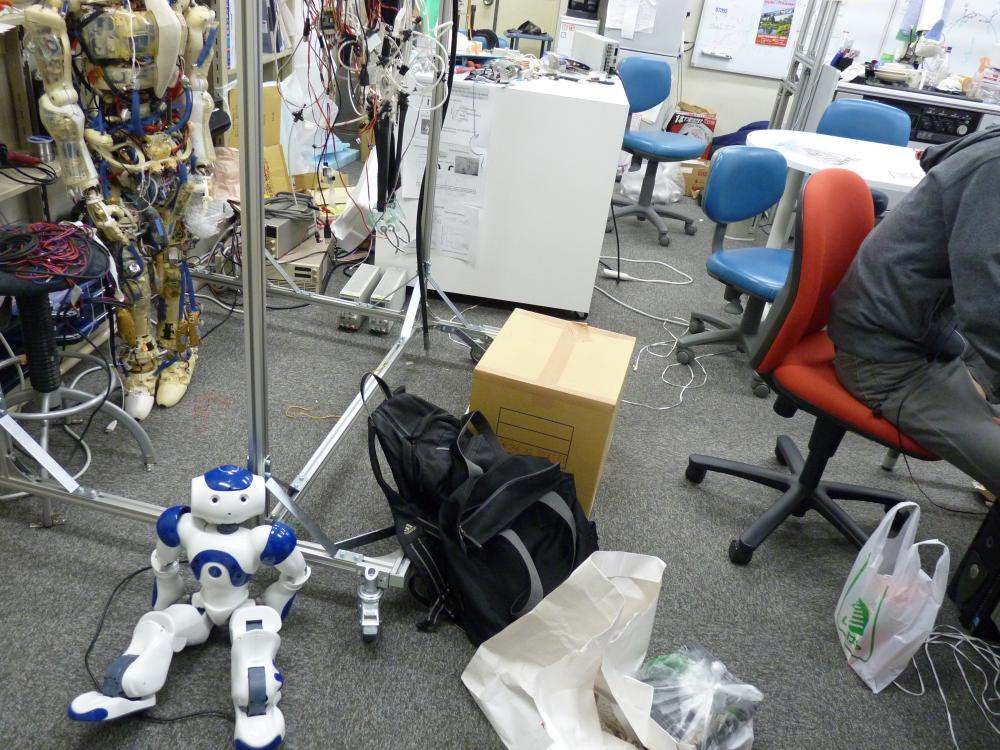
\includegraphics[width=0.50\hsize]{\FIGDIR/photo.jpg}%
    \caption{図の貼り方}%
    \label{fig:lab}%
  \end{center}%
\end{figure}%
図\ref{fig:lab}はこのようにして貼られた図である.
図に対して言及するときはこのようにrefコマンドを使う.
refコマンドの引数を,図を貼った時のコマンド群中のlabelコマンドの引数と対応させることで,意図した図に対してrefすることができるのである.

さて,先ほどの図の貼り方はちょっとめんどくさい.
大体,たかが図を一枚貼るためにこんな数行使った処理をいちいち書いてられないし,ソースコードのスペース的にもたくさん消費してしまってアホみたいである.
そのあたりを解決するのが,figコマンドである.
(figコマンドはいわば自作関数で,ikuo.styの中に定義されている.)
figコマンドを使うと,下記のように図を貼ることができる.
\fig{photo.jpg}{width=.50\hsize}{figコマンドを使って貼った図}
\figref{photo.jpg}はfigコマンドを使って貼った図である.
そして,今,気づいただろうか.
今のrefはただのrefではなく,figrefコマンドを使ってrefを行ったものである.
(figrefコマンドもfigコマンド同様にikuo.styの中で定義されている.)
figrefコマンドを使うと,いちいち「図」とか「fig.」とかをrefコマンドの前に書く必用がなくなり,便利である.
更に,「図」でなく「fig.」として参照するように変更する必用が生じた時にも,ikuo.styの中のfigrefコマンドの定義箇所にて変更をするだけで文書全体に変更が行われるのでとても有用であり,figrefコマンドを使わないのは愚かしい行為である.


\subsection{figに関連する便利コマンド}

figコマンドには残念ながら,図の位置を指定する引数が存在しない.
figコマンドの定義を見ると,位置指定オプションは[tbp]となっており,ページ上端,下端,まるまる1ページ,という優先度で位置が指定されることがわかる.
どうしてもページ下端に図を貼りたいんだ,という時にはfigbコマンドが用意されている.
\figb{photo2.jpg}{width=.50\hsize}{figbコマンドを使って貼った図}
\figref{photo2.jpg}はfigbコマンドを使って貼った図である.

どうしても位置を自分で指定したい,という場合はfigposコマンドを使う.
figposコマンドは第4引数が位置指定オプションに反映されるため,下記のように使うことができる.
\figpos{photo3.jpg}{width=.50\hsize}{figposコマンドを使って貼った図}{t}
\figref{photo3.jpg}はfigposコマンドを使って貼った図である.

上記各コマンドと合わせ,定義されているfig関連のコマンドを以下にまとめておく.
\begin{itemize}
\item fig\\
  図を貼るときに使う一番基本的なコマンド.
  位置指定は[tbp]となる.
  
\item twofigs\\
  2枚の図を立てに並べて貼るときに使うコマンド.
  キャプションは1つだけつき,ラベルは最初の図のファイル名になる.
  位置指定は[tbp]となる.
  
\item figthroug\\
  複数段組の文書中で,段組をぶちぬいて図を貼るときに使うコマンド.
  
\item figb\\
  ページ下端に図を貼るときに使うコマンド.
  
\item figpos\\
  任意の位置を指定して図を貼るときに使うコマンド.
  
\item doublefig\\
  2枚の図を横に並べて貼るときに使うコマンド.
  キャプションは1つだけつき,ラベルは最初の図のファイル名になる.
  位置指定は[tb]となる.
  
\item doublefigt\\
  doublefigコマンドと同様だが,ページ上端に図を貼るとき専用のコマンド.
  具体的には図の上側にスペースを入れずに貼ることができる.
  
\item doublefigb
  doublefigコマンドと同様だが,ページ下端に図を貼るとき専用のコマンド.
  
\item doublefigthrough\\
  doublefigコマンドと同様だが,複数段組の文章中で段組をぶちぬいて図を貼るときに使うコマンド.
  位置指定は[t]となる.
  
\item triplefig\\
  3枚の図を横に並べて貼るときに使うコマンド.
  キャプションは1つだけ表示され,ラベルは最初の図のファイル名になる.
  位置指定は[tbp]となる.
  
\item triplefigthrough\\
  triplefigコマンドと同様だが,複数段組の文章中で段組をぶちぬいて図を貼るときに使うコマンド.
  位置指定は[tbp]となる.
  
\end{itemize}


\section{表と式の書き方}
\seclabel{table_equation}

\subsection{表の書き方}
表を書くときには以下のようにする.
\begin{table}[tb]
  \label{sample}
  \begin{center}
    \caption{各人データ}
    \begin{tabular}{l|c|c|r}
      \hline
      名前 & 身長[cm] & 体重[kg] & 備考 \\
      \hline
      Y.M & 1800 & 60 & \\
      Y.M & 170 & 10 & \\
      Y.M & 170 & 60 & はげ\\
      \hline
    \end{tabular}
  \end{center}
\end{table}
表\ref{sample}は最も基本的な表の書き方の例である.
ソースコードを見ればわかる通り,この中ではlabelコマンドが使われているのだが,より便利なコマンドとしてtablabelが用意されている.
tablabelコマンドは表に対するラベルであるという情報をを自動的に付与してくれるため,これを用いることで図や式に対するラベルとごっちゃになるという問題を防ぐことができる.
同様のコマンドとしてfiglabel(図に対するラベル),equlabel(式に対するラベル),chaplabel(章に対するラベル),seclabel(節に対するラベル),subseclabel(小節に対するラベル)などが存在するので使うと良い.
\secref{fig}において用いたfigだとかtwofigだとかいった便利コマンドにおいてはその中でfiglabelが使用されている.

tablabelコマンドを用いた表は以下のようになる.
\begin{table}[tb]
  \tablabel{sample2}
  \begin{center}
    \caption{各人データ}
    \begin{tabular}{l|c|c|r}
      \hline
      名前 & 身長[cm] & 体重[kg] & 備考 \\
      \hline
      Y.M & 1800 & 60 & \\
      Y.M & 170 & 10 & \\
      Y.M & 170 & 60 & はげ\\
      \hline
    \end{tabular}
  \end{center}
\end{table}
\tabref{sample2}のようにtablabelを用いて表を書くと,tabrefコマンドを使うのが便利になる.
tabrefコマンドはfigrefコマンドのように自動で「図」とか「table」とかをつけてくれる便利コマンドである.

表に関しては特にこれ以上ローカルなコマンドとかないので,あとは研究室wikiを見るなりネットで情報探すなりして自分の書きたい表を書けるようになってください.


\subsection{式の書き方}
式は例えば以下のように書く.
\begin{eqnarray}
  \equlabel{hoge}
  hoge=hage
\end{eqnarray}

式に関してここで述べるべきことは表に関するそれとほぼ同様であり,つまりequlabelおよびequrefを使うべきであるという点のみである.
\equref{hoge}はequlabelを使ってラベル付されており,本文章冒頭のrefはequrefを用いて行われている.
式の書き方に関するそれ以外の情報は研究室wikiなりネット上で情報探すなりしてください.

ahaha

\addcontentsline{toc}{chapter}{謝辞}
\markboth{謝辞}{謝辞}
\chapter*{謝辞}
卒業論文を執筆するに当たり,水内郁夫教授より多大なるご指導,ご鞭撻を賜りました.
多くの技術,知識をこの一年間で学ばせていただきました.深く感謝申し上げます.
また,森下克幸助教にも論文執筆や発表技術に関するアドバイスをいただき,
Professor Tom{\'a}{\v{s} Vyhl{\'\i}dal,Mr. Juraj Lieskovsk{\`y}をはじめ,
Czech Technical University in Pragueの皆様には
留学時に多くのアドバイスをいただき,英語が不安な私をサポートしてくださいました.
感謝申し上げます.
さらに,研究室の先輩,同期には研究の面,そして研究以外の面でも支えていただきました.
本当にありがとうございました.


% \begin{verbatim}
% %% \addcontentsline{toc}{chapter}{謝辞}
% %% \markboth{謝辞}{謝辞}
% %% \chapter*{謝辞}
卒業論文を執筆するに当たり,水内郁夫教授より多大なるご指導,ご鞭撻を賜りました.
多くの技術,知識をこの一年間で学ばせていただきました.深く感謝申し上げます.
また,森下克幸助教にも論文執筆や発表技術に関するアドバイスをいただき,
Professor Tom{\'a}{\v{s} Vyhl{\'\i}dal,Mr. Juraj Lieskovsk{\`y}をはじめ,
Czech Technical University in Pragueの皆様には
留学時に多くのアドバイスをいただき,英語が不安な私をサポートしてくださいました.
感謝申し上げます.
さらに,研究室の先輩,同期には研究の面,そして研究以外の面でも支えていただきました.
本当にありがとうございました.


% \begin{verbatim}
% %% \addcontentsline{toc}{chapter}{謝辞}
% %% \markboth{謝辞}{謝辞}
% %% \chapter*{謝辞}
卒業論文を執筆するに当たり,水内郁夫教授より多大なるご指導,ご鞭撻を賜りました.
多くの技術,知識をこの一年間で学ばせていただきました.深く感謝申し上げます.
また,森下克幸助教にも論文執筆や発表技術に関するアドバイスをいただき,
Professor Tom{\'a}{\v{s} Vyhl{\'\i}dal,Mr. Juraj Lieskovsk{\`y}をはじめ,
Czech Technical University in Pragueの皆様には
留学時に多くのアドバイスをいただき,英語が不安な私をサポートしてくださいました.
感謝申し上げます.
さらに,研究室の先輩,同期には研究の面,そして研究以外の面でも支えていただきました.
本当にありがとうございました.


% \begin{verbatim}
% %% \addcontentsline{toc}{chapter}{謝辞}
% %% \markboth{謝辞}{謝辞}
% %% \include{thanks}
% \end{verbatim}

% emacs の人は、M-x comment-region ですね。
% コメント解除は、C-u M-x comment-region ですね。


% \end{verbatim}

% emacs の人は、M-x comment-region ですね。
% コメント解除は、C-u M-x comment-region ですね。


% \end{verbatim}

% emacs の人は、M-x comment-region ですね。
% コメント解除は、C-u M-x comment-region ですね。



\addcontentsline{toc}{chapter}{参考文献}
\markboth{参考文献}{参考文献}
\bibliographystyle{junsrt}
\bibliography{reference}

\end{document}
